\documentclass[10pt,a4paper]{report}
\usepackage[latin1]{inputenc}
%\usepackage[utf8x]{inputenc}
\usepackage{amsmath}
\usepackage{amsfonts}
\usepackage{amssymb}
\usepackage{graphicx}


\begin{document}
	Alban Pierre
	\newline
	20th January 2017
	\newline
	\begin{center}
		\textbf{\Large{Topic C : seeing the arrow of time}}
		\newline
	\end{center}
	
	\section*{Introduction}
	
	Humans can see if a video is running forward or backward, like in the following 3 images we can easily tell that it is backward.
	\newline
	\begin{figure}[h]
		\begin{minipage}[b]{.30\linewidth}
			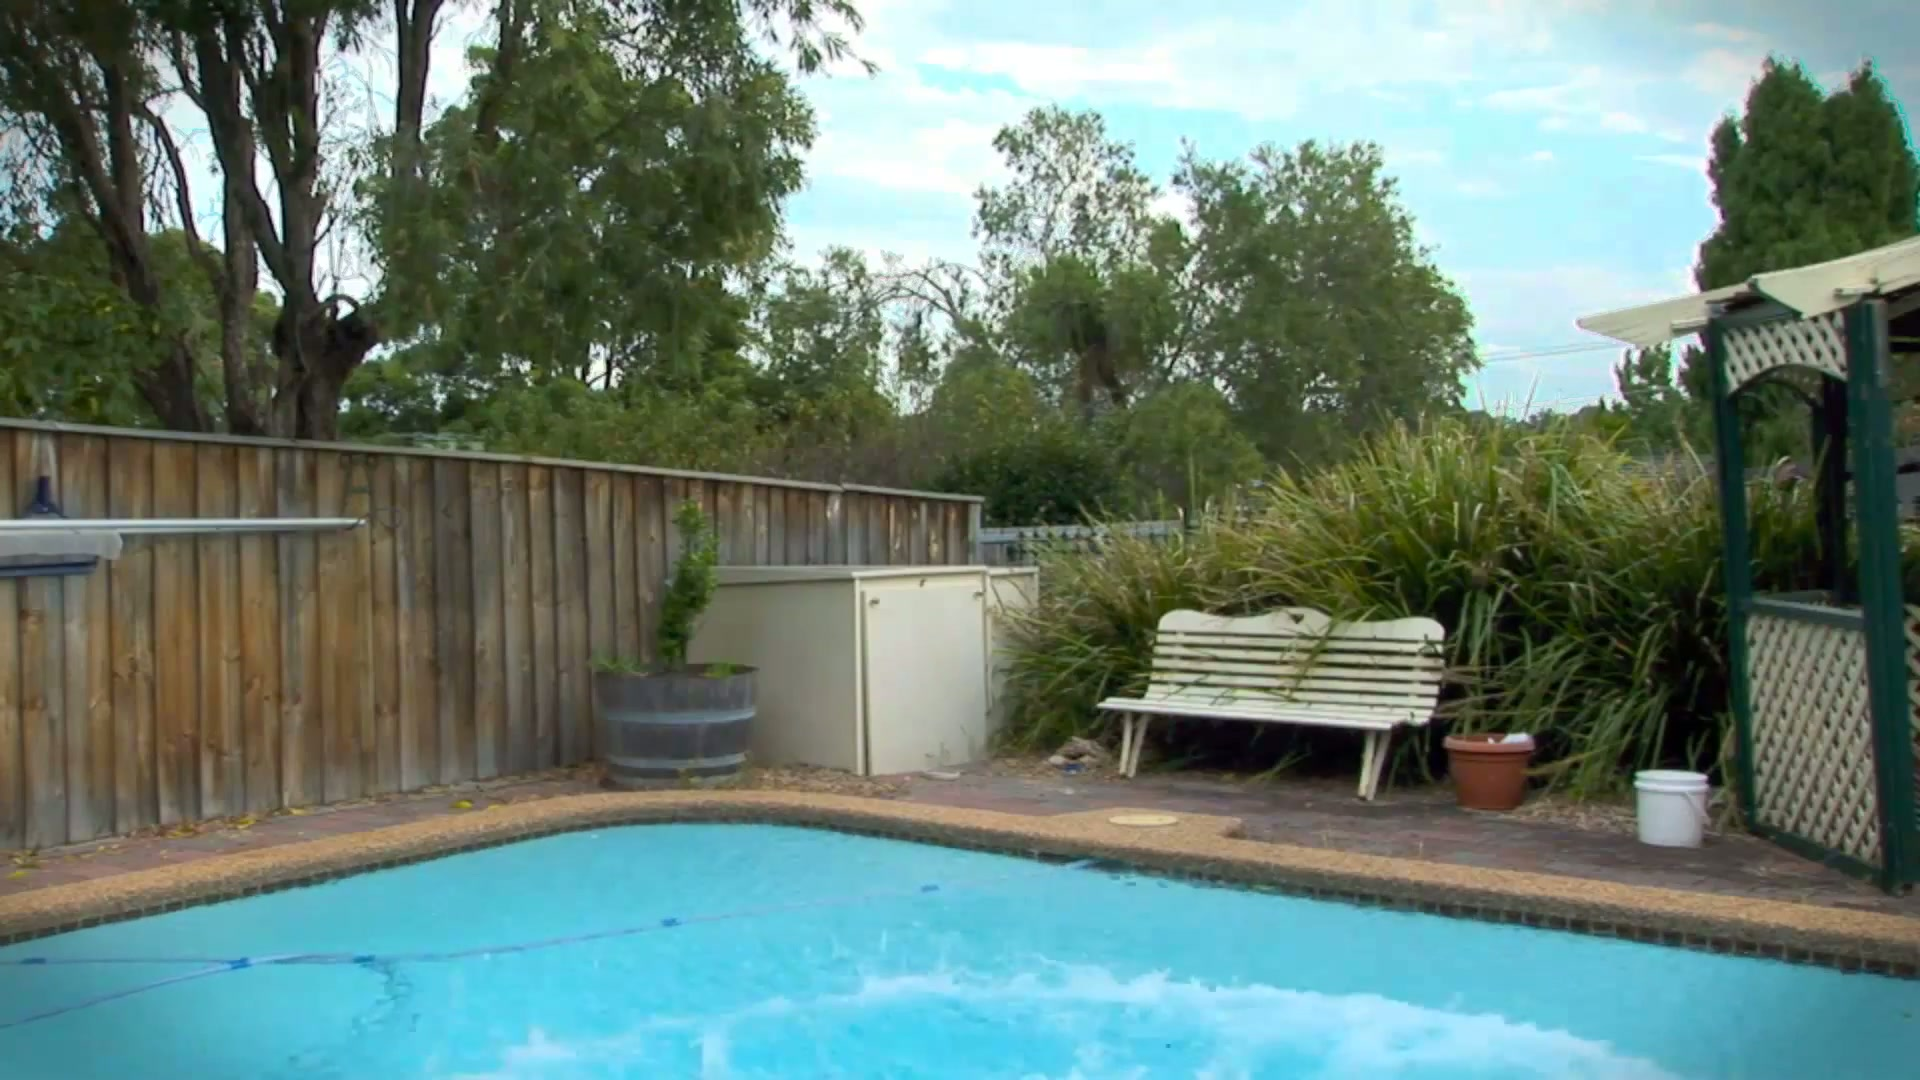
\includegraphics[width=1.0\textwidth]{im01.jpeg}
			%\caption{1000 first iterations (3*2, one)}
		\end{minipage}
		\hspace{5pt}
		\begin{minipage}[b]{0.30\linewidth}
			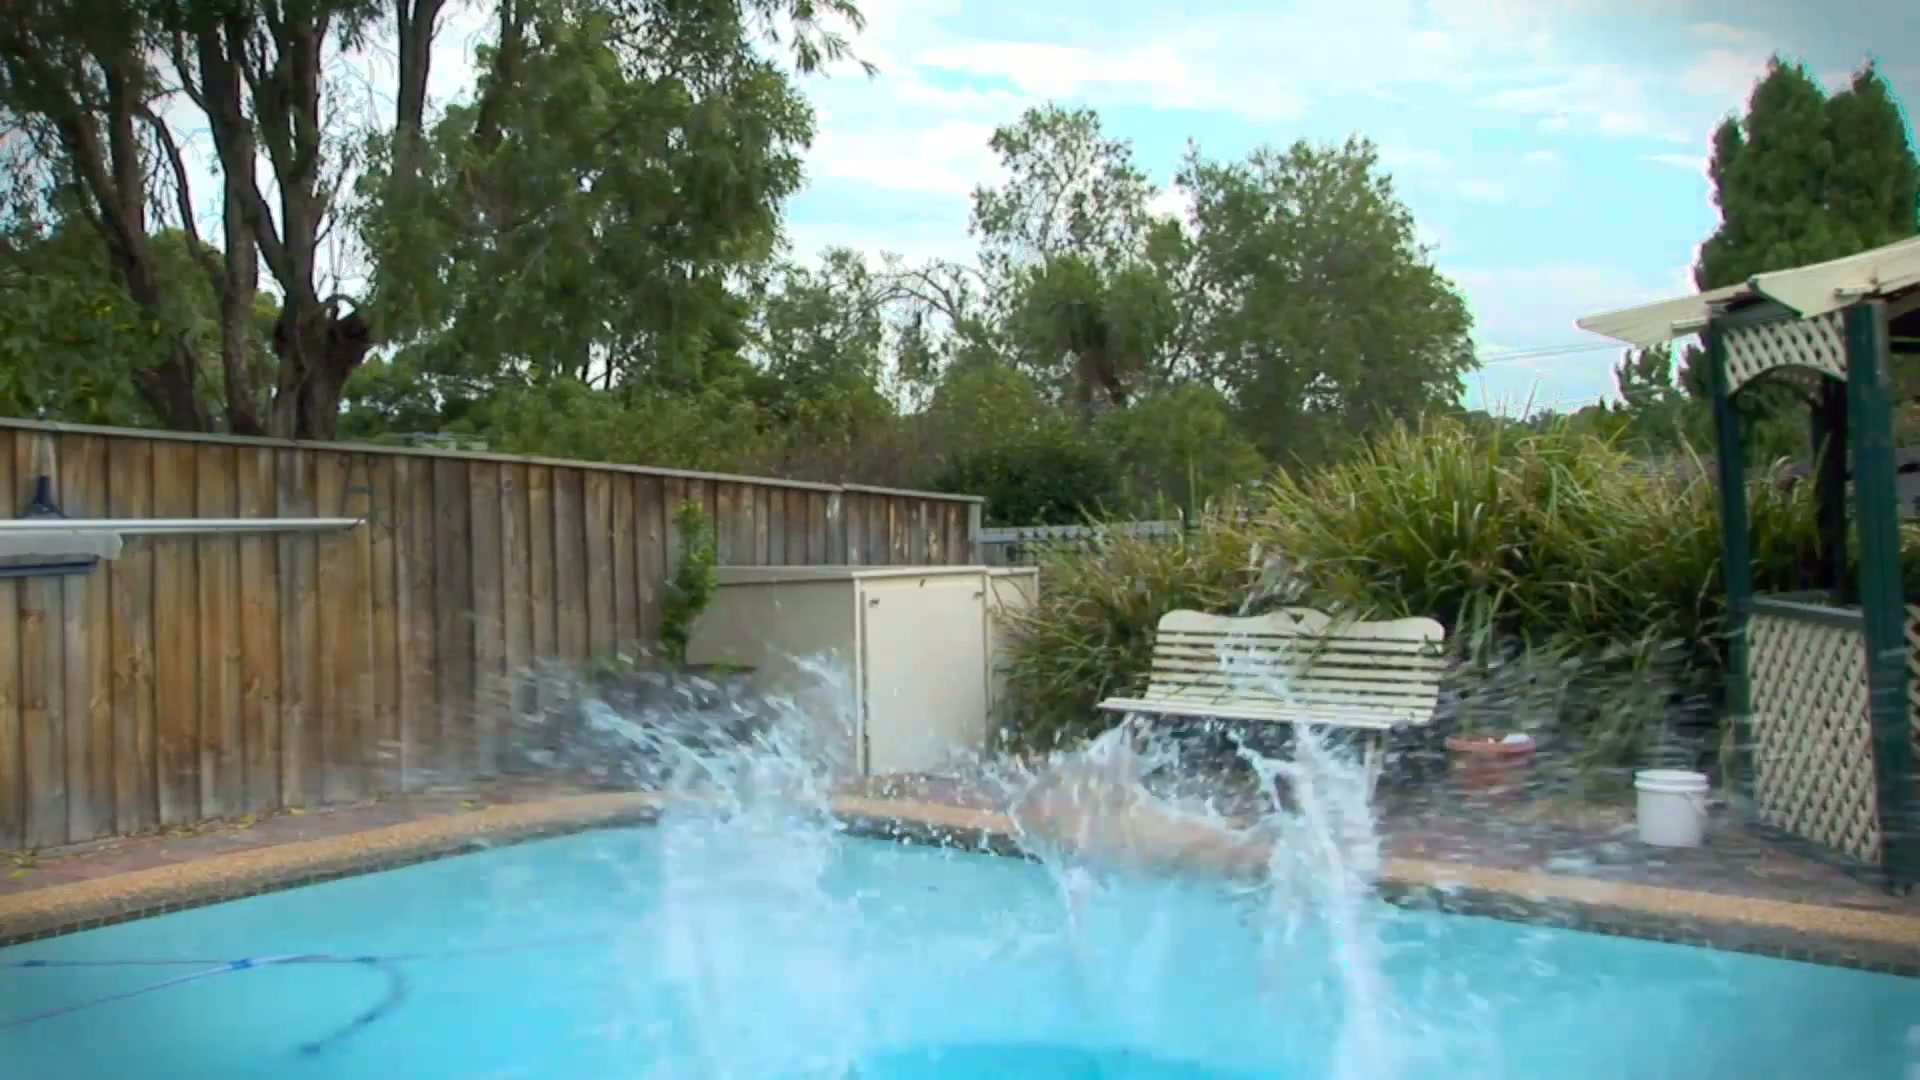
\includegraphics[width=1.0\textwidth]{im30.jpeg}
			%\caption{1000 last iterations (3*2, one)}
		\end{minipage}
		\hspace{5pt}
		\begin{minipage}[b]{0.30\linewidth}
			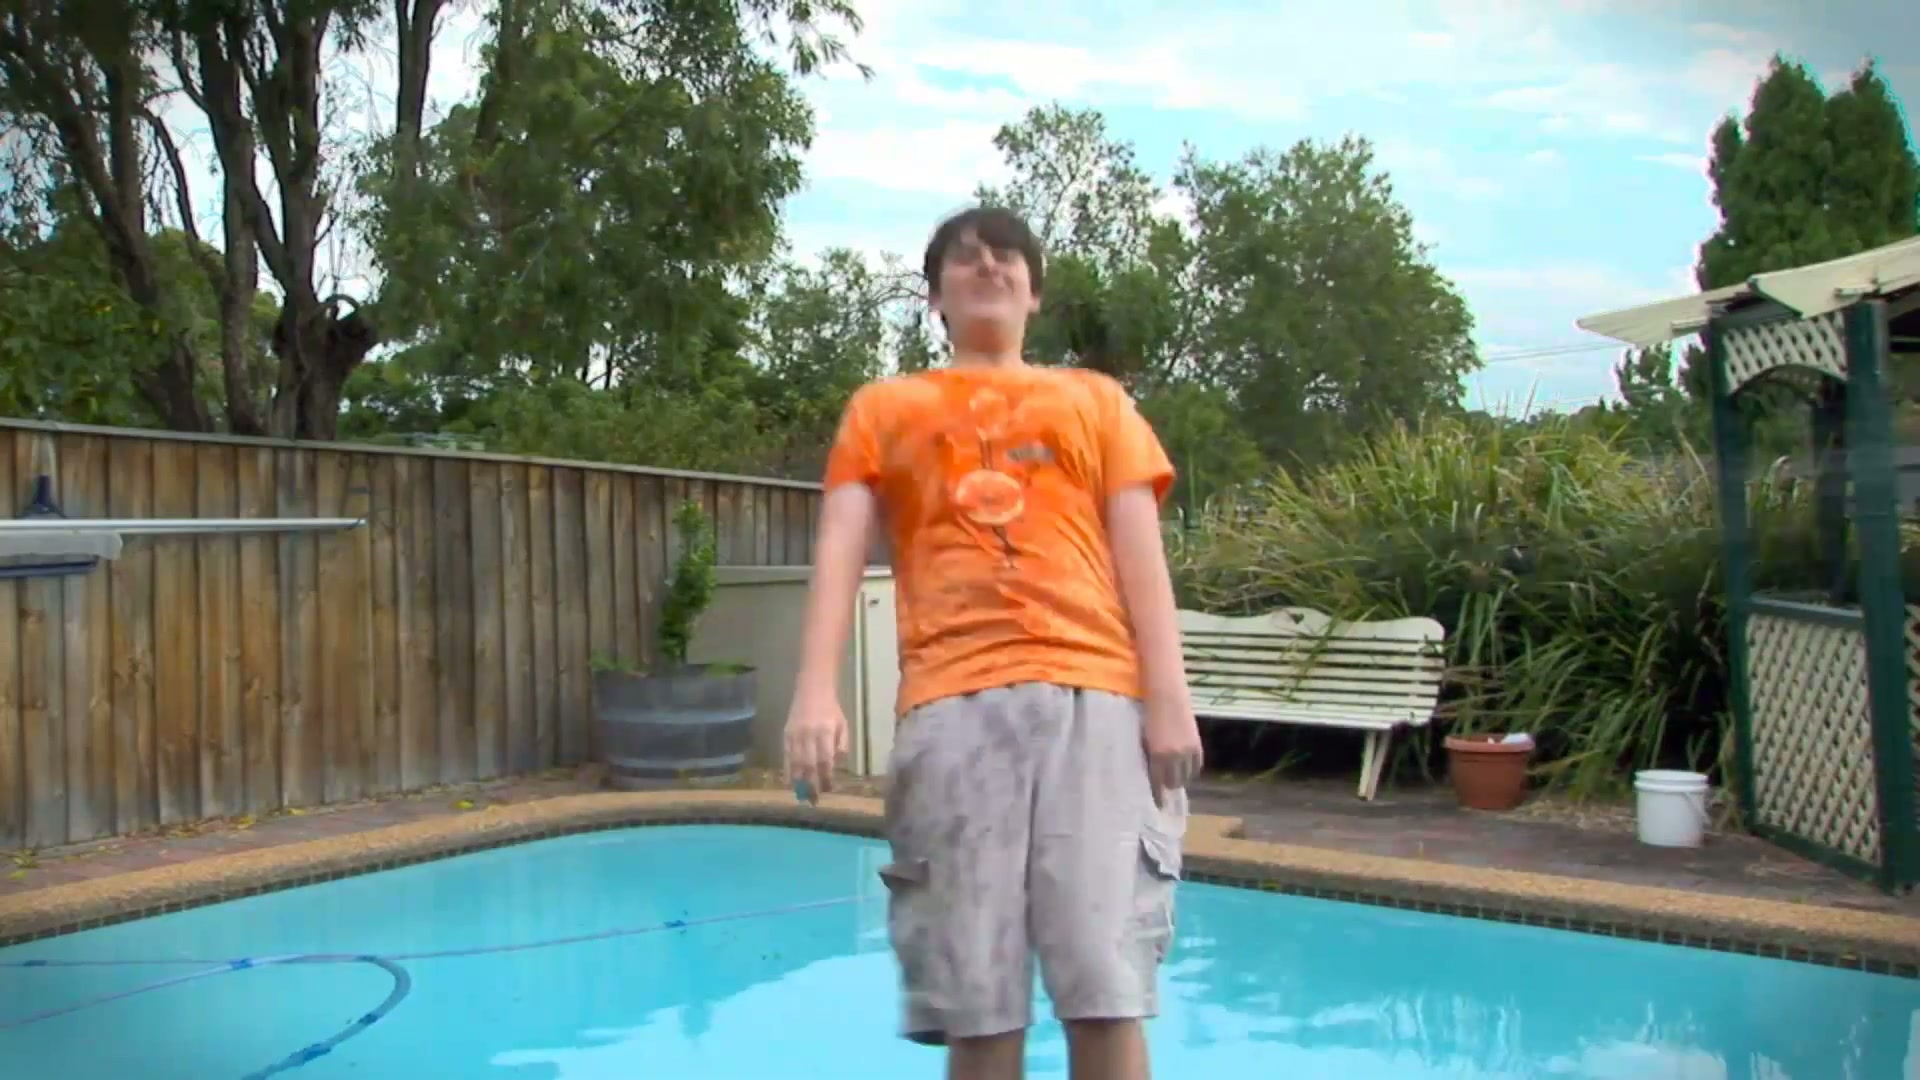
\includegraphics[width=1.0\textwidth]{im50.jpeg}
			%\caption{1000 last iterations (3*2, one)}
		\end{minipage}
		\label{fig:f}
	\end{figure}
	
	Following the article [1], I tried to implement an algorithm that tackle this problem.
	
	\section*{General structure of the algorithm}
	
		The first step is to compute descriptors, there are many ways to do this so I explain it in details in the next section.
		
		Then given these descriptors, we have to reduce the size of each video representation (there are many descriptors by video), so I run a k-means algorithm to get only the $K$ most used descriptors and I assign each descriptor to his closest descriptor computed by k-means. Then we can represent each video by a vector of size $K$ where at index $k$ there is the number of occurrences of descriptor $k$.
		
		In other words, we have constructed histograms that represent videos. Eventually I run an SVM classifier on these histograms (normalized). I used the barrier method to compute the SVM.
	
		\section*{Computation of descriptors}
		
		This is the main choice of the algorithm, as we have to compute descriptors that contains information about the arrow of time. For this I could have chosen to use pre-trained convolutionnal neural networks, but these networks were pre-trained for an other task which means they could have lost information about the arrow of time, or simply be not efficient.
		
		So I choose to compute motion descriptors based on optical flow, and then train my own CNN.  
		
		\subsection*{Motion descriptors based on optical flow}
		
		I firstly implemented optical flow descriptors based on the Horn \& Schunck algorithm [3]. They assumes that
		\begin{itemize}
			\item $f(x,y,t) = f(x+dx, y+dy, t+dt)$ (Assumes brightness constancy)
			\item $f(x+dx,y+dy,t+dt) = f(x,y,z) + \frac{\partial f}{\partial x}dx + \frac{\partial f}{\partial y}dy + \frac{\partial f}{\partial t}dt$ (Assumes small motions)
		\end{itemize}
		in order to get an algorithm that only iterates the following equations :
		\[u = u_{av} - fx\frac{fx u_{av} + fy v_{av} + ft}{\alpha + fx^2 + fy^2}\]
		\[v = v_{av} - fy\frac{fx u_{av} + fy v_{av} + ft}{\alpha + fx^2 + fy^2}\]
		The two following figures are the optical flow that I obtained from the first image of this report (and her next frame) :
		\begin{figure}[h]
			\begin{minipage}[b]{.49\linewidth}
				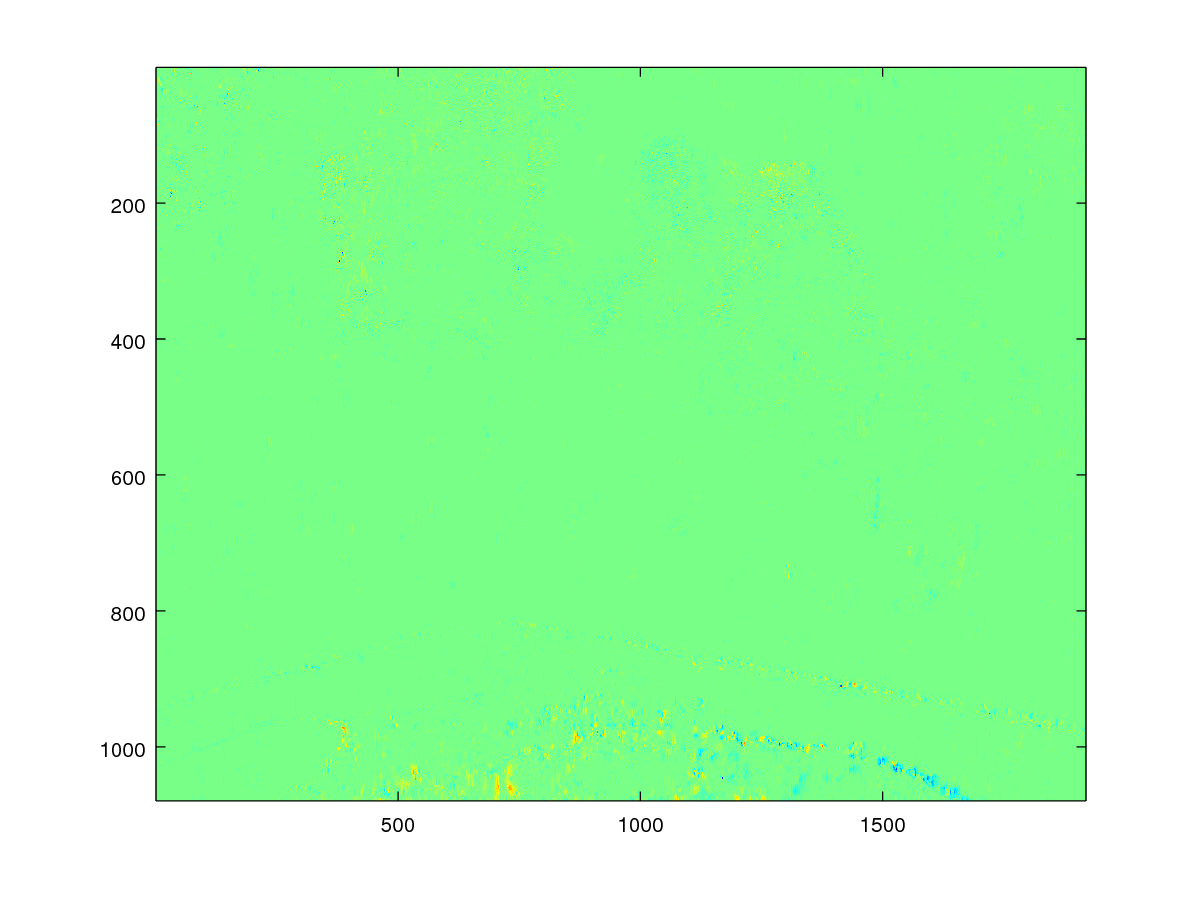
\includegraphics[width=1.0\textwidth]{ofx.png}
				\centering{Opt. flow along the $x$ axis}
			\end{minipage}
			\hfill
			\begin{minipage}[b]{0.49\linewidth}
				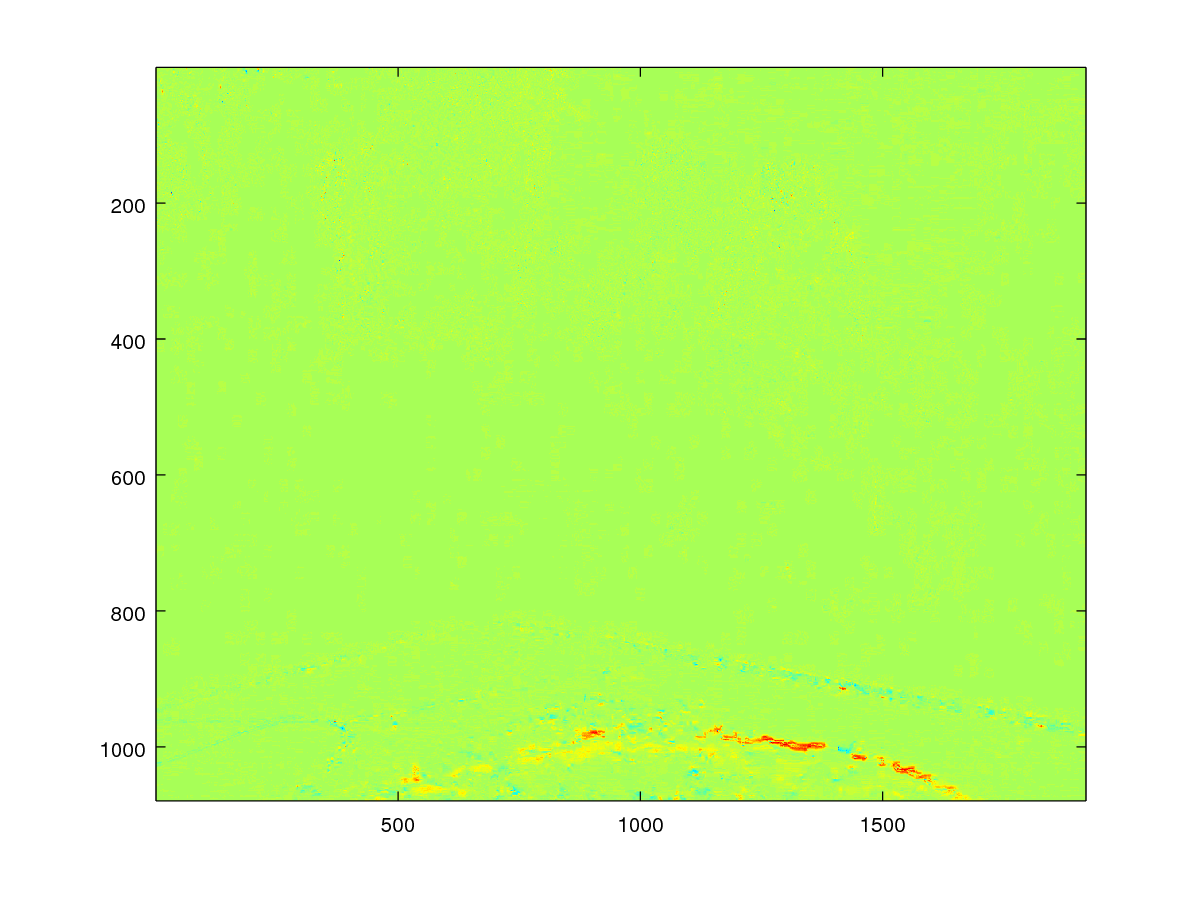
\includegraphics[width=1.0\textwidth]{ofy.png}
				\centering{Opt. flow along the $y$ axis}
			\end{minipage}
			\label{fig:f}
		\end{figure}
		
		In practice this algorithm does not get motion for big objects, but only the motions of its borders. So I tried to implement a better algorithm [4], it basically computes Horn \& Schunck optical flow for different resolutions of an image, wrapping the coarse image result into a finer one. But it relies on a difficult warpping algorithm that I could not get right, and as the subject was more on CNN I abandoned this optical flow computation to focus on CNN.
		
		\subsection*{Convolution Neural Network descriptors}
		
		I tried to use the architectures presented in [2, 5, 6]. The goal of [2] is that recognizing if frames are in a good temporal order or not forces the CNN to recognize the arrow of time. The goal of [5] is that motions of objects (like explosions) gives many informations about the arrow of time, and computing the segmentation helps a lot in computing motions. The algorithm in [6] serve just as a reference.
		
		Unfortunately the time of training for simpler structures was too long and I could not train any of the previous architectures. Then I tried to use 3 dimensional CNN. The idea was that subsampling in time whithin the 3D CNN is a gain in time (this subsampling in time is inexistant in the previous architectures where we take the video frame by frame). But here again the training phase was too long.
		
		I recoded partially the DeepLearnToolbox by R. B. Palm [7] to create the 3D CNN toolbox.
		
		\section*{Results}
		
			As CNNs cannot be trained properly in a reasonable amount of time, I have only results based on the optical flow descriptors (parameters : the images are subsampled by a factor of 4, I used the 80 first frames of the 180 videos - each also fliped in time - of the dataset of [1], and I used histograms of size 100).
			
			Here are the training and testing results that I got depending on the $C$ parameter of the SVM :
		
		\section*{References}
		\scriptsize{
		\begin{itemize}
			
			\item[*] [1] Pickup, L. C., Pan, Z., Wei, D., Shih, Y., Zhang, C., Zisserman, A., ... \& Freeman, W. T. (2014). Seeing the arrow of time. In Proceedings of the IEEE Conference on Computer Vision and Pattern Recognition (pp. 2035-2042).
			
			\item[*] [2] Misra, I., Zitnick, C. L., \& Hebert, M. (2016, October). Shuffle and learn: unsupervised learning using temporal order verification. In European Conference on Computer Vision (pp. 527-544). Springer International Publishing.
			
			\item[*] [3] Horn, B. K., \& Schunck, B. G. (1981). Determining optical flow. Artificial intelligence, 17(1-3), 185-203.
			
			\item[*] [4] Brox, T., Bruhn, A., Papenberg, N., \& Weickert, J. (2004, May). High accuracy optical flow estimation based on a theory for warping. In European conference on computer vision (pp. 25-36). Springer Berlin Heidelberg.
			
			\item[*] [5] Long, J., Shelhamer, E., \& Darrell, T. (2015). Fully convolutional networks for semantic segmentation. In Proceedings of the IEEE Conference on Computer Vision and Pattern Recognition (pp. 3431-3440).
			
			\item[*] [6] Krizhevsky, A., Sutskever, I., \& Hinton, G. E. (2012). Imagenet classification with deep convolutional neural networks. In Advances in neural information processing systems (pp. 1097-1105).
			
			\item[*] [7] Palm, R. B. (2012). Prediction as a candidate for learning deep hierarchical models of data. Technical University of Denmark, 5.
			
		\end{itemize}
	}
	

\end{document}






